\documentclass[aspectratio=169,12pt]{beamer}
\usepackage{graphicx} % For including graphics.
\usepackage{hyperref} % For links.

\title{Connascence}
\author{Jan Wedekind}
\date{Wednesday, April 9th 2025}

\hypersetup{
   pdftitle          = {Connascence},
   pdfsubject        = {Short presentation about Connascence},
   pdfauthor         = {Jan Wedekind},
   pdfkeywords       = {software, quality, metric, engineering},
   pdfcreator        = {okular},
   pdfproducer       = {LaTeX with hyperref and thumbpdf},
   bookmarksopen     = false,
   bookmarksnumbered = true,
   colorlinks        = true,
}

\usebackgroundtemplate{
\includegraphics[width=\paperwidth,height=\paperheight]{slide}}

\begin{document}

\frame{\titlepage}

\begin{frame}
  \frametitle{Motivation}
  \begin{itemize}
    \item Metric for software quality
    \item Theoretical foundation for software engineering
  \end{itemize}
\end{frame}

\begin{frame}
  \frametitle{Talk(s) by Jim Weirich}
  \begin{center}
    \href{https://www.youtube.com/watch?v=q85rdBMe9GY}{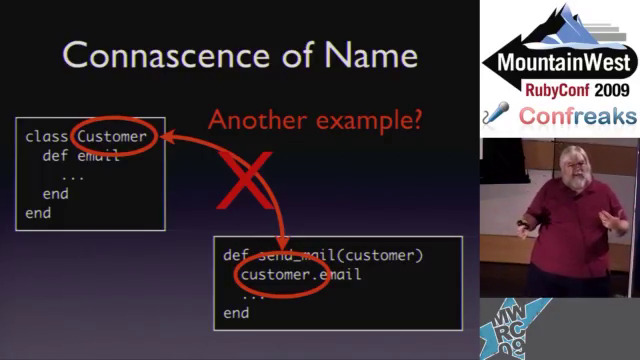
\includegraphics[height=.8\textheight]{weirich}}
  \end{center}
\end{frame}

\begin{frame}
  \frametitle{Book by Meilir Page-Jones}
  \begin{center}
    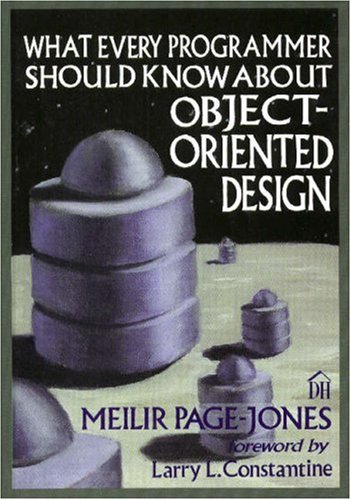
\includegraphics[height=.8\textheight]{meilir}
  \end{center}
\end{frame}

\begin{frame}
  \frametitle{Connascence Definition}
  Jim Weirich:\bigskip\\
  \begin{quote}
    Two pieces of software share \textbf{connascence} when a change in one requires a corresponding change in the other.
  \end{quote}
\end{frame}

\end{document}
